% Panel (c): Segmentation — content only, no tikzpicture
% Stacked transparent layers with actual segmentation contours
% Draw order: back to front (base → iris → pupil → edges → labels)

\pgfmathsetmacro{\imgw}{1.1}
\pgfmathsetmacro{\imgh}{0.6875}
\pgfmathsetmacro{\offx}{0.18}
\pgfmathsetmacro{\offy}{0.18}

% The base layer (layer0) defines the pipeline y
\pgfmathsetmacro{\basey}{-0.55*\panelH}
\coordinate (stackbase) at (0.28*\panelW, \basey);

% RITnet at same y as layer0
% CNN label above
\node[font=\scriptsize\sffamily, text=segteal!70!black]
  at (0.07*\panelW, \basey + 0.75) {CNN};

% CNN block (taller, same width)
\node[segblock, minimum width=1.4cm, minimum height=1.1cm]
  at (0.07*\panelW, \basey) (ritnet) {};

% Mini CNN layers: 3D-ish slices
\begin{scope}[shift={($(ritnet.center)+(-0.42, 0)$)}, scale=0.85]
  \fill[segteal!20] (0, -0.35) rectangle ++(0.14, 0.7);
  \fill[segteal!30] (0, 0.35) -- ++(0.14, 0) -- ++(0.06, 0.06) -- ++(-0.14, 0) -- cycle;
  \fill[segteal!25] (0.14, -0.35) -- ++(0, 0.7) -- ++(0.06, 0.06) -- ++(0, -0.7) -- cycle;
  \fill[segteal!30] (0.28, -0.28) rectangle ++(0.14, 0.56);
  \fill[segteal!40] (0.28, 0.28) -- ++(0.14, 0) -- ++(0.06, 0.06) -- ++(-0.14, 0) -- cycle;
  \fill[segteal!35] (0.42, -0.28) -- ++(0, 0.56) -- ++(0.06, 0.06) -- ++(0, -0.56) -- cycle;
  \fill[segteal!40] (0.56, -0.20) rectangle ++(0.13, 0.40);
  \fill[segteal!50] (0.56, 0.20) -- ++(0.13, 0) -- ++(0.05, 0.05) -- ++(-0.13, 0) -- cycle;
  \fill[segteal!45] (0.69, -0.20) -- ++(0, 0.40) -- ++(0.05, 0.05) -- ++(0, -0.40) -- cycle;
  \fill[segteal!50] (0.82, -0.12) rectangle ++(0.11, 0.24);
  \fill[segteal!60] (0.82, 0.12) -- ++(0.11, 0) -- ++(0.04, 0.04) -- ++(-0.11, 0) -- cycle;
  \fill[segteal!55] (0.93, -0.12) -- ++(0, 0.24) -- ++(0.04, 0.04) -- ++(0, -0.24) -- cycle;
\end{scope}

% === LAYER 0: Base image (backmost) ===
\node[inner sep=0.5pt, draw=stemgrey!40, thin]
  at (stackbase) (layer0)
  {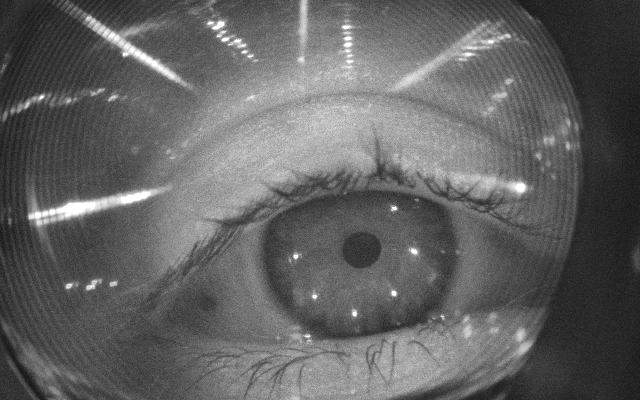
\includegraphics[width=\imgw cm]{preprocessed_eye.png}};

% === LAYER 1: Iris box + contour ===
\node[inner sep=0.5pt, draw=blue!40, thin,
  minimum width=\imgw cm, minimum height=\imgh cm, fill=white, fill opacity=0.6]
  at ($(stackbase)+(\offx, \offy)$) (layer1) {};

\draw[blue!80, semithick, fill=blue!15, fill opacity=0.4, shift={(layer1.south west)}]
  plot[smooth cycle] coordinates {(0.6273,0.3609) (0.6050,0.3575) (0.5878,0.3558) (0.5758,0.3523) (0.5552,0.3506) (0.5448,0.3472) (0.5363,0.3455) (0.5294,0.3420) (0.5208,0.3403) (0.5156,0.3369) (0.5070,0.3352) (0.5019,0.3317) (0.4967,0.3300) (0.4916,0.3266) (0.4847,0.3248) (0.4795,0.3214) (0.4709,0.3180) (0.4623,0.3077) (0.4606,0.3025) (0.4572,0.2956) (0.4555,0.2853) (0.4520,0.2750) (0.4538,0.2320) (0.4572,0.2234) (0.4589,0.2097) (0.4623,0.2011) (0.4641,0.1925) (0.4692,0.1856) (0.4727,0.1788) (0.4795,0.1702) (0.4864,0.1598) (0.5070,0.1375) (0.5156,0.1323) (0.5259,0.1238) (0.5311,0.1220) (0.5363,0.1186) (0.5414,0.1169) (0.5483,0.1134) (0.5534,0.1117) (0.6016,0.1083) (0.6273,0.1100) (0.6394,0.1134) (0.6548,0.1152) (0.6652,0.1186) (0.6755,0.1203) (0.6841,0.1238) (0.7030,0.1255) (0.7116,0.1289) (0.7219,0.1306) (0.7288,0.1341) (0.7339,0.1409) (0.7477,0.1547) (0.7580,0.1667) (0.7597,0.1719) (0.7631,0.1770) (0.7648,0.1822) (0.7683,0.1873) (0.7700,0.1942) (0.7734,0.2028) (0.7752,0.2114) (0.7786,0.2200) (0.7803,0.2303) (0.7838,0.2406) (0.7820,0.2784) (0.7786,0.2888) (0.7769,0.2991) (0.7734,0.3059) (0.7717,0.3145) (0.7683,0.3197) (0.7666,0.3266) (0.7631,0.3334) (0.7597,0.3369) (0.7528,0.3386) (0.7459,0.3420) (0.7373,0.3438) (0.7305,0.3472) (0.7202,0.3489) (0.7133,0.3523) (0.6978,0.3541) (0.6841,0.3575) (0.6480,0.3592)};

% === LAYER 2: Pupil box + contour (frontmost) ===
\node[inner sep=0.5pt, draw=green!50!black, thin,
  minimum width=\imgw cm, minimum height=\imgh cm, fill=white, fill opacity=0.6]
  at ($(stackbase)+(2*\offx, 2*\offy)$) (layer2) {};

\draw[green!70!black, semithick, fill=green!15, fill opacity=0.5, shift={(layer2.south west)}]
  plot[smooth cycle] coordinates {(0.6136,0.2888) (0.6084,0.2870) (0.6050,0.2853) (0.6016,0.2836) (0.5947,0.2750) (0.5930,0.2716) (0.5913,0.2664) (0.5895,0.2544) (0.5913,0.2458) (0.5930,0.2423) (0.6033,0.2338) (0.6067,0.2320) (0.6291,0.2303) (0.6325,0.2320) (0.6359,0.2338) (0.6411,0.2372) (0.6480,0.2458) (0.6514,0.2527) (0.6531,0.2681) (0.6514,0.2733) (0.6480,0.2784) (0.6411,0.2836) (0.6377,0.2853) (0.6325,0.2870)};

% === EDGE LINES ===
\draw[stemgrey!25, thin] (layer0.north west) -- (layer2.north west);
\draw[stemgrey!25, thin] (layer0.south west) -- (layer2.south west);
\draw[stemgrey!25, thin] (layer0.south east) -- (layer2.south east);

% === LABELS (between stack and ellipse fit, vertically stacked) ===
% x position: midway between layer2.east and ellipse.west
\pgfmathsetmacro{\labelx}{0.28*\panelW + 2*\offx + 0.5*\imgw + 0.01}
\node[font=\tiny\sffamily\itshape, text=green!60!black, anchor=west]
  at (\labelx, \basey + 2*\offy + 0.16) {pupil};
\node[font=\tiny\sffamily\itshape, text=blue!70, anchor=west]
  at (\labelx, \basey + \offy + 0.16) {iris};
\node[font=\tiny\sffamily\itshape, text=stemgrey!60, anchor=west]
  at (\labelx, \basey + 0.16) {input};

% === Ellipse fit — same y as layer0 ===
\node[segblock] at (0.60*\panelW, \basey) (ellipse) {Ellipse\\Fit};

% Small arrowhead style for fan-out
\tikzset{
  smallarr/.style={-{Stealth[length=2.5pt,width=2pt]}, thin, color=segteal!70!black},
}

% Fan-out: centred on ellipse fit y
\pgfmathsetmacro{\fanx}{0.82*\panelW}
\pgfmathsetmacro{\fansp}{0.45}
\node[segoutlabel, minimum width=1.3cm] at (\fanx, \basey + 1.5*\fansp) (seg_pupil) {Pupil diameter};
\node[segoutlabel, minimum width=1.3cm] at (\fanx, \basey + 0.5*\fansp) (seg_iris) {Iris diameter};
\node[segoutlabel, minimum width=1.3cm] at (\fanx, \basey - 0.5*\fansp) (seg_centre) {Pupil centre};
\node[segoutlabel, minimum width=1.3cm] at (\fanx, \basey - 1.5*\fansp) (seg_conf) {Confidence};

% === ARROWS ===
% RITnet → layer0 (horizontal, same y)
\draw[segarr] (ritnet) -- (layer0);
% Stack → ellipse fit (horizontal from layer2.east at basey)
\draw[segarr] (layer2.east |- layer0.east) -- (ellipse.west);
% Fan-out
\draw[smallarr] (ellipse.east) -- ++(0.12,0) |- (seg_pupil.west);
\draw[smallarr] (ellipse.east) -- ++(0.12,0) |- (seg_iris.west);
\draw[smallarr] (ellipse.east) -- ++(0.12,0) |- (seg_centre.west);
\draw[smallarr] (ellipse.east) -- ++(0.12,0) |- (seg_conf.west);
